\documentclass[12pt]{article}
\usepackage[margin=0.9in]{geometry} 
\usepackage[utf8]{inputenc}
\usepackage{amsmath}
\usepackage{amsfonts}
\usepackage{amssymb}
\usepackage{graphicx}
\usepackage{color}
\usepackage{float}
\usepackage{scrextend}
\usepackage{enumitem}
\usepackage{parskip}
\usepackage{siunitx}
%\usepackage{listings}

%ignore \hbox issue
\hfuzz=100pt

% title declarations
\newcommand{\doctitle}{Project 5 - Finite State Machine Layout}
\newcommand{\docsubtitle}{FSM Layout and Design Problems}
\newcommand{\docsubsub}{Width = $\SI{0.875}{\mu m}$, Length = $\SI{2.085}{\mu m}$\\ Area = $\SI{1.8244}{\mu m^2}$ Delay = $\SI{59.3223}{ps}$\\ Area * Delay = $\SI{108.226}{}$ }

\renewcommand{\maketitle} {
    \setlength{\parindent}{0pt}
    \begin{center} \
        % top spacing
        \vspace*{1in}

        % main title
        \huge{\doctitle}\\
        \Large{\docsubtitle}\\

        % naming
        \vspace*{0.2in}
        \large{
            Arthur Hsueh\\
            21582168\\
            UBC - ELEC 402
        }
    \end{center}
}

\begin{document}
\maketitle
\thispagestyle{empty}
\pagebreak

\tableofcontents
\thispagestyle{empty}
\pagebreak

\listoffigures
\thispagestyle{empty}

\listoftables
\thispagestyle{empty}

\pagebreak
\setcounter{page}{1}
\section{Finite State Machine Layout}                       % Q1
\subsection{Review of FSM Design - Assignment 1 \& 2}
The finite state machine (FSM) design was the one used in Assignments 1 and 2. The detailed design of the FSM is too long for the purpose of this report, so this section will reiterate the General Description of the design and functionality of the FSM from Assignment 1.

"My finite state machine (FSM) is a simplified application of a credit card payment controller. It accepts payment in the form of VISA, MasterCard or AMEX, and includes basic operations that one would see when paying with a credit card. 

The state machine moves through the states of card association selection, confirmation of payment, pin processing and processing the actual payment. It also includes state transitions when confirmation of payment, pin processing and actual payment processing fails. As a more unique feature, I added in a fail counter for the pin processing, allowing the state machine to abort processing if the user enters their pin incorrectly too many times.

The FSM assumes a more modular design, and functions as a controller to the whole system. The unique inputs of the FSM are bits that trigger transitions to new states, and the outputs of the FSM are bits that function as enables to other modules."

For detailed input/outputs of the FSM as well as the testbench design used to simulate the FSM, please refer to my Assignment 1.

Because we are using the \_map.v file generated by the synthesis tool of Cadence, the design name now includes an appended \_map on each corresponding file.
% FSM Function
% Input/Outputs
% Testing procedure
\subsection{Virtuoso Layout} % virtuoso image with rules
Below is the image of the transistor layout of the FSM. The placement and routing of the design was first performed in the Encouter software, and then imported into Virtuoso.
\begin{figure} [H]
    \centering
    \makebox[\textwidth]{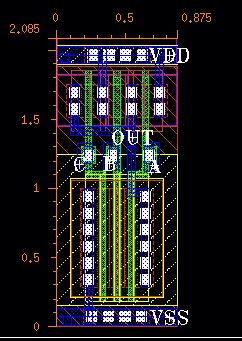
\includegraphics[scale=0.7]{../images/q1_layout.jpg}}
    \caption{credit\_card\_payment\_FSM\_map layout}
\end{figure}

Rulers have been added to show the dimensions of the layout. The table below shows the dimensions and the resulting area.
\begin{table} [H]
    \centering
    \begin{tabular}{ccc}
        Width & Length &  Area\\
        \hline
        $\SI{21.1}{\mu m}$ & $\SI{22.8}{\mu m}$ & $\SI{281.08}{\mu m^2}$
    \end{tabular}
    \caption{Dimensions of the FSM Circuit}
\end{table}

\subsection{Verification of Layout} % Modelsim waveforms with new sdf
To verify the functionality of the FSM circuit, I generated a new .sdf file from Encounter and used it to simulate the testbench used in Assignment 1. A Modelsim project was created and the testbench file, Assignment 2 \_map file and the gpdk045 basic cell file was added. The testbench instantiates the \_map module and runs with the .sdf file created in Encounter. The waveform is plotted and the output of the testbench will indicate any errors. Below is the waveform generated from the simulation.
\begin{figure} [H]
    \centering
    \makebox[\textwidth]{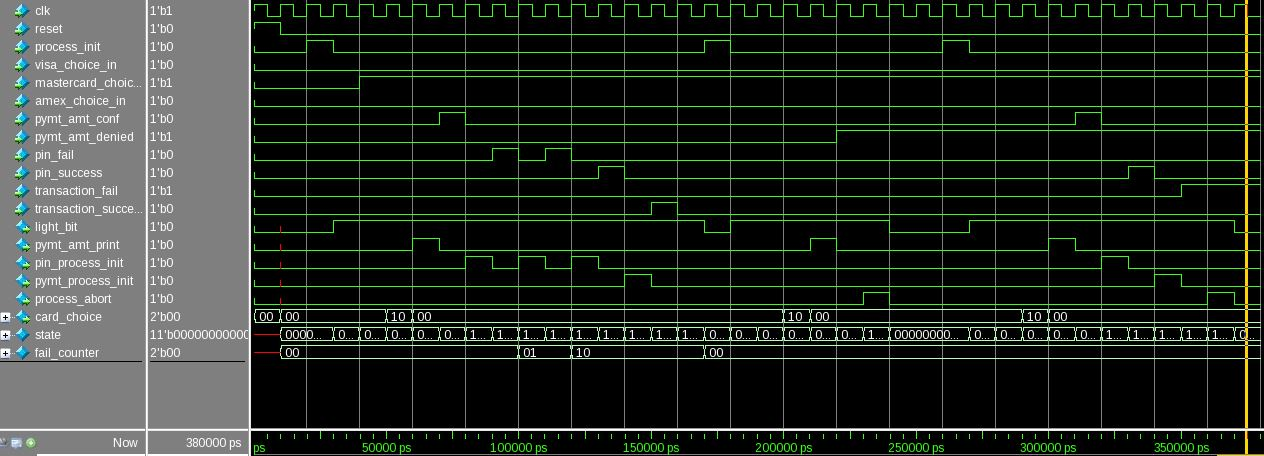
\includegraphics[scale=0.6]{../images/q1_tb_waveform.jpg}}
    \caption{credit\_card\_payment\_FSM\_map layout}
\end{figure}
Compared against the waveform generated in Assignment 1, it is exactly the same. This is supported by the fact that all assertions made in the testbench were evaluated to be true, and no errors were reported.

\subsection{Testing verification}
\subsubsection{Verilog Netlist}
The verilog netlist is the new \_map file generated from Encounter, and not from the original synthesis. The code is too long to include in the report while maintianing its original formatting integrity, so it is attached with the report. The file is credit\_card\_payment\_fsm\_map.v.

\subsubsection{.sdf File} % produced by encounter in the PnR Folder
The .sdf file is generated by Encounter as well. Again, the code is too long to include in the report while maintianing its original formatting integrity, so it is attached with the report. The file is credit\_card\_payment\_fsm.sdf.

\subsubsection{Geometry Check} % from encounter
The geometry check is performed to check against all design rules. Below is both the terminal output from the test, as well as the contents of the outputted .rpt file. The .rpt file is attached with this report, named credit\_card\_payment\_fsm\_map.geom.rpt.
\begin{figure} [H]
    \centering
    \makebox[\textwidth]{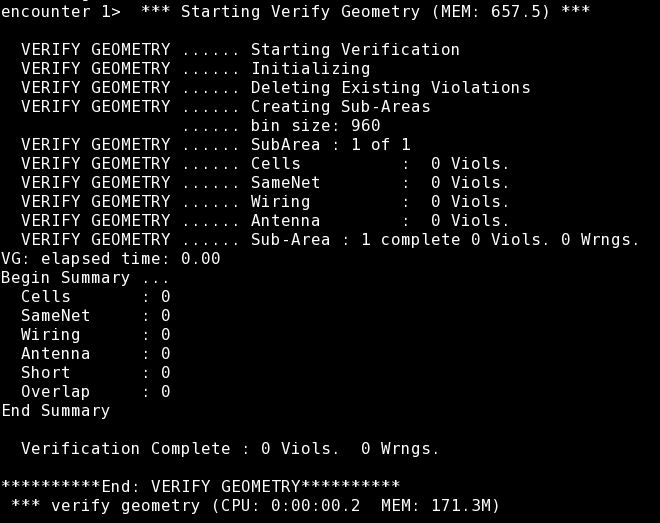
\includegraphics[scale=0.7]{../images/q1_geometry_verify.jpg}}
    \caption{Terminal output for the Geometry Check}
\end{figure}

\begin{figure} [H]
    \centering
    \makebox[\textwidth]{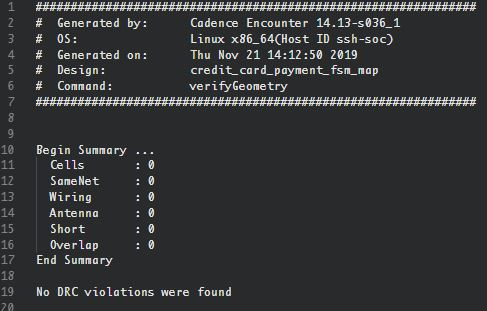
\includegraphics[scale=0.8]{../images/q1_geometry_rpt.jpg}}
    \caption{.rpt Contents for the Geometry Check}
\end{figure}

\subsubsection{DRC Check} % from encounter
The DRC check is performed to check against all design rules like the geometry check. Below is both the terminal output from the test, as well as the contents of the outputted .rpt file. The .rpt file is attached with this report, named credit\_card\_payment\_fsm\_map.drc.rpt.
\begin{figure} [H]
    \centering
    \makebox[\textwidth]{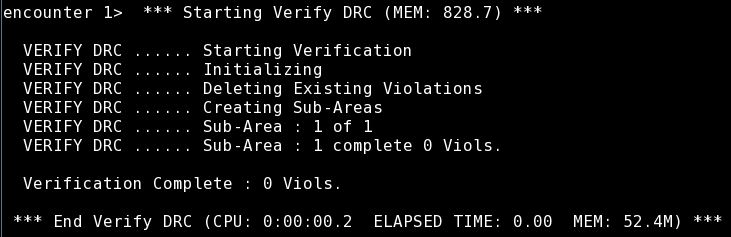
\includegraphics[scale=0.7]{../images/q1_drc_verify.jpg}}
    \caption{Terminal output for the DRC Check}
\end{figure}


\begin{figure} [H]
    \centering
    \makebox[\textwidth]{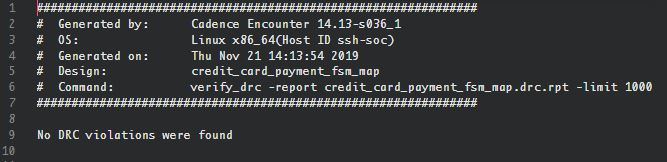
\includegraphics[scale=0.8]{../images/q1_drc_rpt.jpg}}
    \caption{.rpt Contents for the DRC Check}
\end{figure}

\subsubsection{Connectivity Check} % from encounter
The connectivity check is performed to check for any missing connections. Below is both the terminal output from the test, as well as the contents of the outputted .rpt file. The .rpt file is attached with this report, named credit\_card\_payment\_fsm\_map.conn.rpt.
\begin{figure} [H]
    \centering
    \makebox[\textwidth]{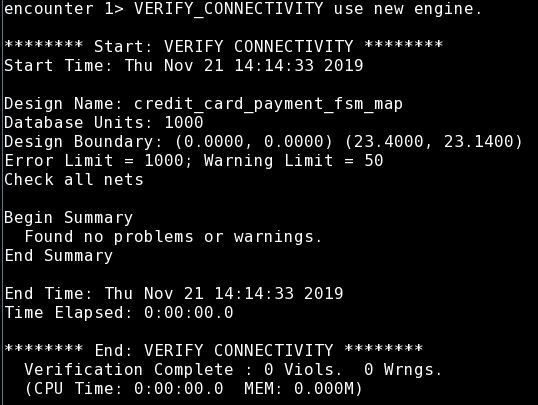
\includegraphics[scale=0.7]{../images/q1_connectivity_verify.jpg}}
    \caption{Terminal output for the Connectivity Check}
\end{figure}
\begin{figure} [H]
    \centering
    \makebox[\textwidth]{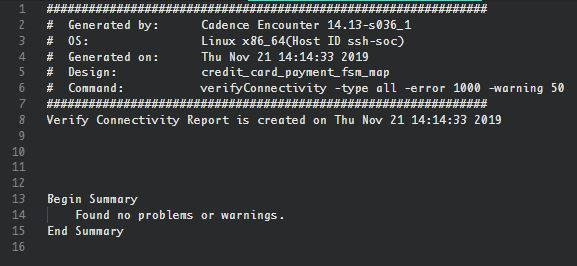
\includegraphics[scale=0.8]{../images/q1_connectivity_rpt.jpg}}
    \caption{.rpt Contents for the Connectivity Check}
\end{figure}


\pagebreak
\section{Domino Logic Problem}                              % Q2
\subsection{Determining the logic function of OUT}
The circuit shown in the logic applies the properties of Domino Logic with the PMOS and NMOS with input 'phi' begint the input clock. OUT is not defined in the circuit, but it is taken as the output of the output inverter. 

The logic of the circuit can be derived by looking at the pull down network NMOS with inputs A, B, C, and D. The parallel C and D NMOS represents an OR, and the series A, B and C and D, NMOS repesents AND. The important note is that the pull down NMOS network represents the \textit{dual} of the origin logic, and the application of the inverter ensures that the ouptut corresponds to the original logic. So, the resulting logic fucntion is 
\[OUT = AB(C+D) \]
\subsection{Voltage Reduction under worst case conditions}
The first step is to determine the input combination with the worst charge sharing. This combination is 
\[ ABCD = 1100 \]
The next step is the calculate the capacitances as the respective nodes. The image below labels the nodes XYZ that will be used for calculation
\begin{figure} [H]
    \centering
    \makebox[\textwidth]{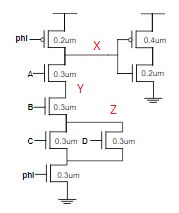
\includegraphics[scale=1]{../images/q2_circuit.jpg}}
    \caption{Problem 2 circuit with labelled nodes}
\end{figure}
For calculations the values $C_{eff}$ and $C_g$ will be used at the declared values of
\[C_{eff} = \SI{1}{fF \mu m^{-1}} \quad and \quad C_g = \SI{2}{fF \mu m^{-1}}\]

\textbf{For $C_X$}

Capacitance at node X is the sum of the effective capacitances of the phi PMOS and A NMOS as well as the gate capacitance at the input of the inverter.
\[C_X = C_{eff}W_{phi} + C_{eff}W_A + C_g(W_p + W_n)\]
\[C_X = \SI{1.7}{fF} \]

\textbf{For $C_Y$}

Capacitance at node X is the self capacitance of the B NMOS.
\[C_X = C_{eff}W_{B}\]
\[C_X = \SI{0.3}{fF} \]

\textbf{For $C_Z$}

Capacitance at node X is the sum of the self capacitances of the C and D NMOS.
\[C_X = C_{eff}(W_C + W_D)\]
\[C_X = \SI{0.6}{fF} \]

\textbf{For V*}

V* is the resulting voltage across all the nodes with the shared charge. Here the capacitances of B, C and D are all charged at once when A and B are input HIGH. So the charge sharing equation will take into account more than two capcitances; the original charge at node X is equal to the charge at all three nodes once the capacitances are charge. As done in class, the initial voltage is taken to be 1.2V.
\[ V^*(C_X + C_Y + C_Z) = V_{initial}C_X \]
\[ V^* = \frac{V_{initial}C_X}{C_X + C_Y + C_Z}\]
\[ V^* = \frac{1.7*1.2}{1.7 + 0.3 + 0.6}\]
\[ V^* = \SI{0.7846}{V}\]

This value is not reasonable, becuase node Z must have a voltage of at most $V_{DD} - 2V_T = 0.4V$. Thus to calculate the accurate voltage at node X we must find the remaining charge at node X after the charge as been shared.
\[Q_{X remaining} = Q_{X original} - (Q_Y + Q_Z) \]
\[C_XV_{X final} = C_XV_{X original} - (C_Y(V_{DD} - V_T) + C_X(V_{DD} - 2V_T)) \]
\[1.7 * V_{X final} = 1.7*1.2 - (0.3*0.8 + 0.6*0.4)\]
\[V_{X final} = \SI{0.9176}{V}\]

Thus the reduction in voltage at the input of the inverter under the worst case charge sharing condition is 
\[V_{reduction} = V_{DD} - V_{X final} \]
\[V_{reduction} = \SI{0.2823}{V}\]

\pagebreak
\section{Transmission Gate Problem}                         % Q3
Below is a notated image of Figure 4 with nodes labelled to assist with value identification.
\begin{figure} [H]
    \centering
    \makebox[\textwidth]{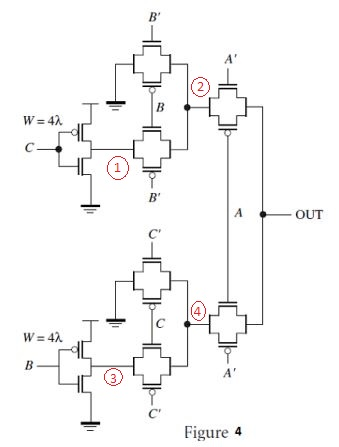
\includegraphics[scale=0.8]{../images/q3_circuit.jpg}}
    \caption{Figure 4 Circuit with annotated nodes}
\end{figure}
\subsection{Capacitance Calculations}
There are 5 nodes in the circuit 1,2,3,4 and OUT. We note that by the nature of the circuit the capacitances at node 3 and 4 are equal to 1 and 2 repsectively.

\textbf{For $C_1$}

The capacitance contributions come from the self capacitance of the PMOS and NMOS of the inverter, the self capacitance of the transmission gate and the gate capcitance of the transmission gate.
\[C_1 = C_{eff-inv-out} + C_{g-TG} + C_{eff-TG} \]
\[C_1 = C_{eff}(W + 2W) + C_g W + 2C_{eff}W \]
\[C_1 = C_3 = 5C_{eff}W + C_g W \]

\textbf{For $C_1$} 

The capcitance contributions come from 3 transmission gates, both the self and gate capacitance.
\[C_2 = 3(C_{g-TG} + C_{eff-TG}) \]
\[C_2 = 3(C_g W + 2C_{eff}W)\]
\[C_2 = C_4 = 6C_{eff}W + 3C_g \]

\textbf{For $C_{out}$}

We are assuming that we are not driving any circuit. Thus the capacitance contributions come from 2 transmission gates.
\[C_{OUT} = 2(C_{g-TG} + C_{eff-TG}) \]
\[C_{OUT} = 2(C_g W + 2C_{eff}W)\]
\[C_{OUT} = 4C_{eff}W + 2C_g \]

For delay calculations we can take the effective resistance of each inverter and gate to be the same as the effective resistance of an NMOS transistor.

\[R = R_{inv} = R_{TG} = R_{nmos} * \frac{L}{W}\]

Delay calculations apply Elmore delay methods.

\subsection{Minimum Delay}
The minimum delay is given by the path from the ground at the input to the most top transmission gate (input 0 of the B-select mux) to OUT. The calculation is as follows.
\[\tau_{min} = C_2*R + C_{OUT}*2R\]
\[\tau_{min} = R(6C_{eff}W + 3C_gW) + 2R(4C_{eff}W + 2C_gW)\]
\[\tau_{min} = RW(14C_{eff} + 17C_g)\]


\subsection{Maximum Delay}
The maximum delay is given by the pathing of Input C to OUT, or Input B to OUT. The calculation is as follows

\[\tau_{max} = \tau_{1} + \tau_{2} + \tau_{OUT}\]
\[\tau_{max} = C_1*R + C_2 * 2R + C_{OUT}*3R\]
\[\tau_{max} = R(5C_{eff}W + C_gW) + 2R(6C_{eff}W + 3C_gW) + 3R(4C_{eff}W + 2C_gW)\]
\[\tau_{max} = RW(29C_{eff} + 13C_g)\]

\subsection{Delay Comparison}
There is no defined technology in the problem, but if we assume a $\SI{0.1}{\mu m}$ technology and the following values 

\[C_{eff} = \SI{1}{fF \mu m^{-1}} \quad and \quad C_g = \SI{2}{fF \mu m^{-1}} \quad and \quad R = \SI{12.5}{k\ohm}\]

Solving for both maximum and minimum delay yields
\[\tau_{min} = \SI{60}{ns} \quad and \quad \tau_{max} = \SI{68.75}{ns} \]

\section{SRAM Cell Problem}                                 % Q4
Not Solved for Submission
\section{FPGA implementation with LUTs}                     % Q5
Not Solved for Submission



\end{document}